\section{Controllers}\label{sec:ContDiscrete}
To implement the controllers, which are designed in the continuous time domain, on the microcontroller they must first be transformed into the discrete time domain.
%The implementation of the controllers can not be done having them as a continuous expression due to the discrete operation of the microcontroller.
%The controllers are expressed in terms of the $z$ operator, the discrete equivalent to the Laplace operator, $s$, from the frequency domain.
This transformation is done through the Tustin (bilinear) approximation in which the $s$ term in the transfer function is substituted as seen in \autoref{tustin} \cite{tustin}.
\begin{flalign}
	s\approx\frac{2}{T}\frac{z-1}{z+1}
	\label{tustin}
\end{flalign}
\begin{where}
	\va{s}{is the Laplace operator}{}
	\va{z}{is the discrete operator}{}
	\va{T}{is the sampling time}{}
\end{where}

The Tustin method maps the Laplace stable region into the discrete stable region, that is, the unit circle, as seen in \autoref{fig:tustinmap}.
\begin{figure}[H]
	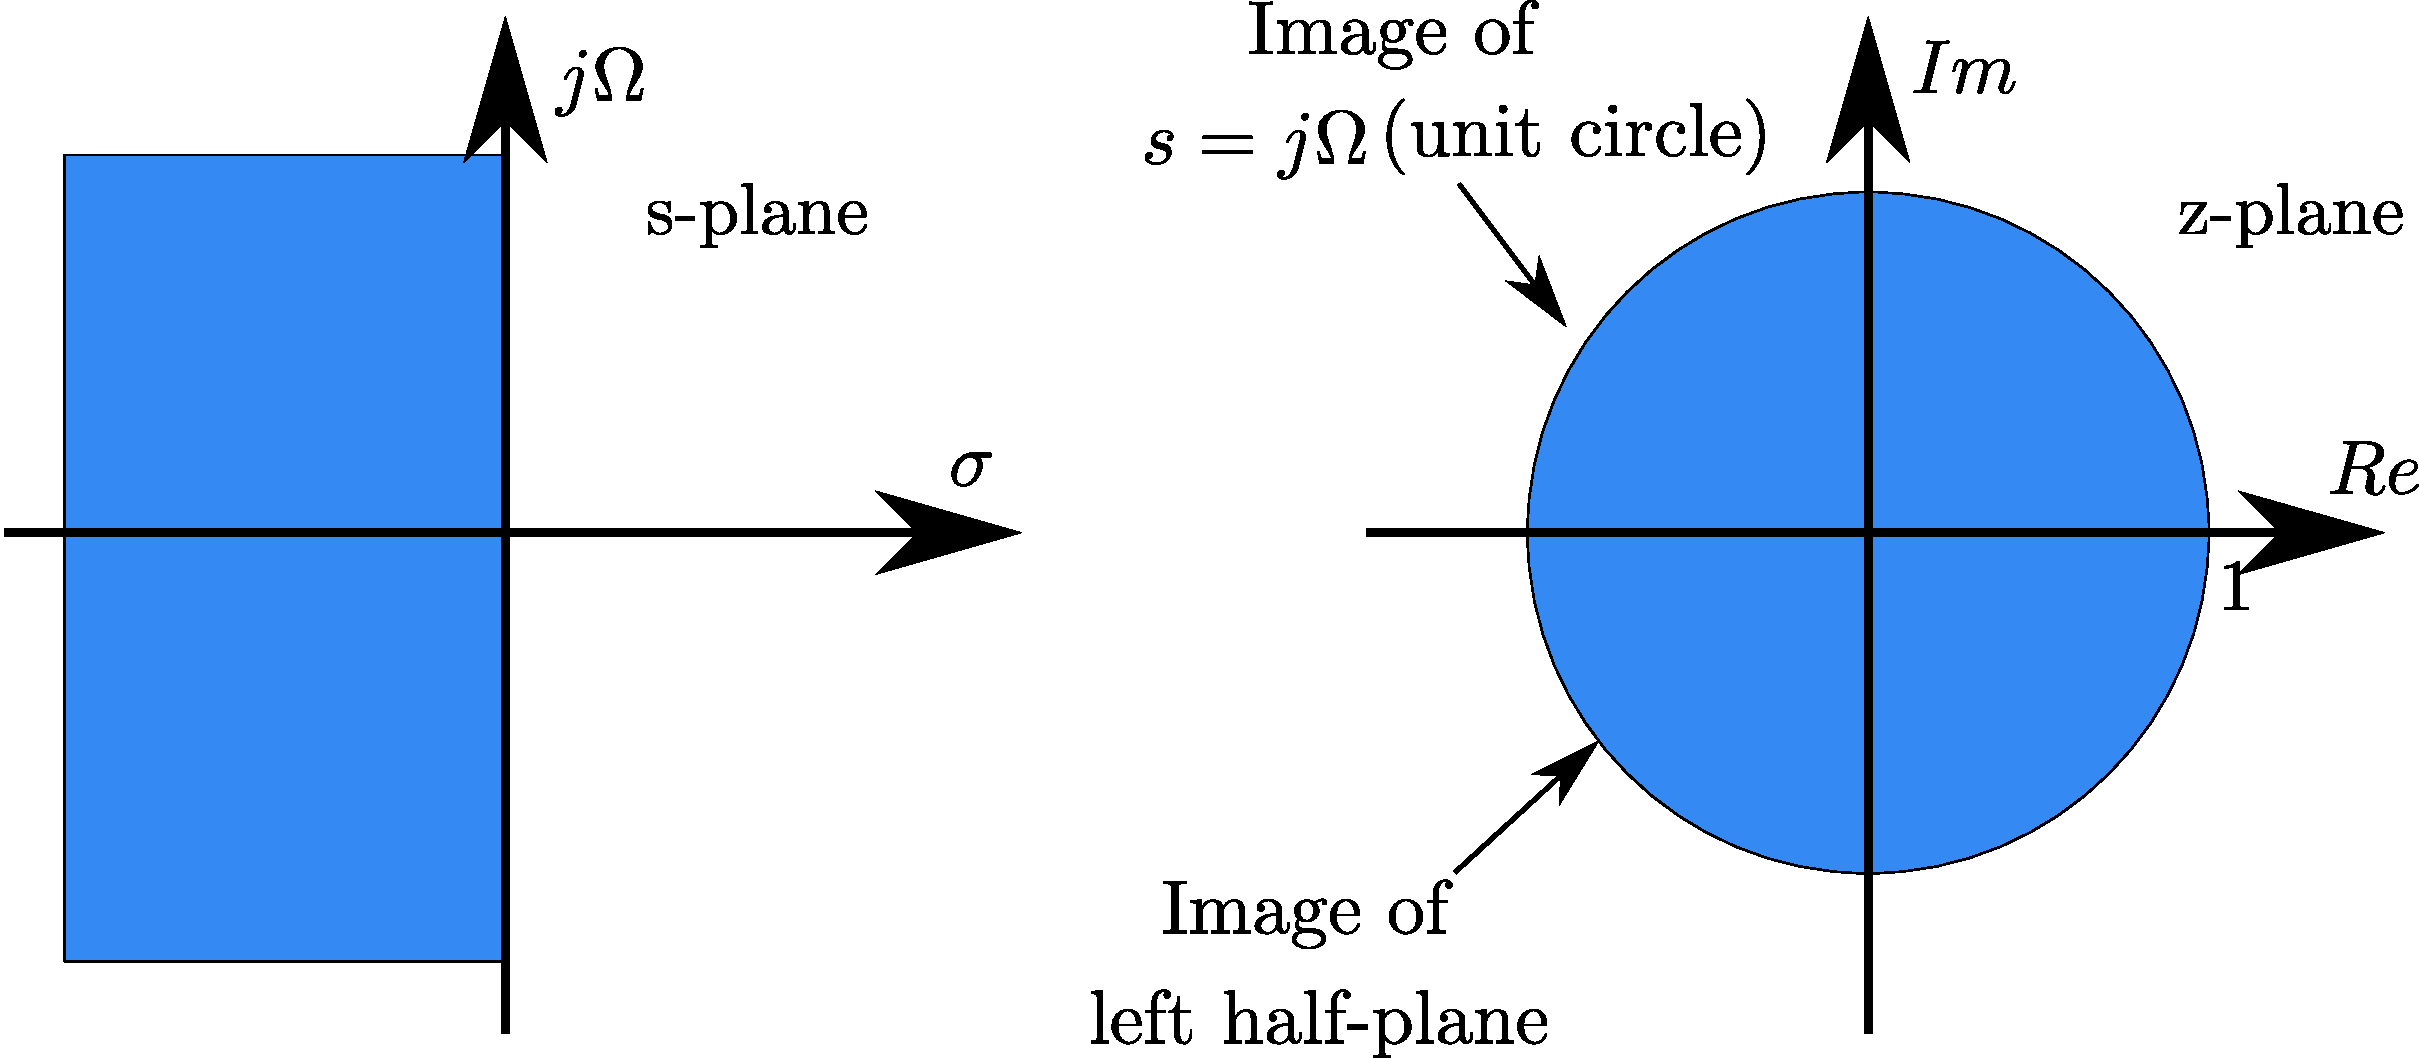
\includegraphics[scale=.3]{figures/SplaneVsZplane.pdf}
	\centering			
	\captionof{figure}{The s-domain and the z-domain \cite{AVOppenheim}.} 
	\label{fig:tustinmap}
\end{figure} 
The discrete transfer function is then transformed into a difference equation to obtain the expression to be applied in the microcontroller. This is done taking into account that a $z^{-1}$ term implies taking the previous sample of the data. 

When discretizing the controller, the sampling time must also be considered. In the system at hand, the sampling frequency is limited by the sensor data (Vicon System) to be 100 Hz as a maximum. The lower limit comes from the bandwidth of the controllers as for the discretization not to affect the controller response, the sampling frequency should from 10 to 20 times higher than the bandwidth of the control loop. The fastest control loop in the system is the attitude controller and has a bandwidth of 5 rad/s, that is, 0.8 Hz. This implies a minimum sampling frequency of 20 Hz.\fxnote{CHECK NUMBERS}

The chosen sampling frequency in the system is 28 Hz in order to keep the controllers with a good performance an far from the 100 Hz that Vicon provides in order to have time for processing the communication and the control tasks.\fxnote{CHECK NUMBERS}

\subsection{Attitude Controller}
The attitude controller is mainly composed of gains formed by the state feedback, the integral and the observer matrices. This makes the discretization easier as there are no $s$ terms in the controller. There are though several integrators, three is in the observer and the other three are placed in the integral part of the controller.

The discrete form of an integrator using the bilinear approximation is shown in \autoref{discreteIntegrator}. The formula shows how the integrator in the integral term of the attitude control looks like when discretized, using the integral control of the roll as example. 
\begin{flalign}
	\frac{x_{int}}{\phi_{ref}-\phi}=\frac{x_{int}}{e_{\phi}} \approx \frac{T}{2}\frac{z+1}{z-1}
	\label{discreteIntegrator}
\end{flalign}

This transformation yields a difference equation as seen in \autoref{discreteIntegratordifferences}. It gives the current value of the integral state as a function of the previous integral state and the current and the previous error between the angular reference and the angular data.
\begin{flalign}
	x_{int}(k)=x_{int}(k-1) + \frac{T}{2} e_{\phi}(k) + \frac{T}{2} e_{\phi}(k-1)
	\label{discreteIntegratordifferences}
\end{flalign}

This approximation is used similarly in the rest of integrators present in the controller.
%The effect of the discretization in the designed attitude controllers has been simulated in the non-linear system and it is commpared with the continuous designed previously developed. See \autoref{fig:AttitudeDiscrete}. It can be seen that the discretized version of the controller makes it slower, but the overshoot is slightly reduced. There no change in the final value of the controller.
%\begin{figure}[H]
%	\centering
%	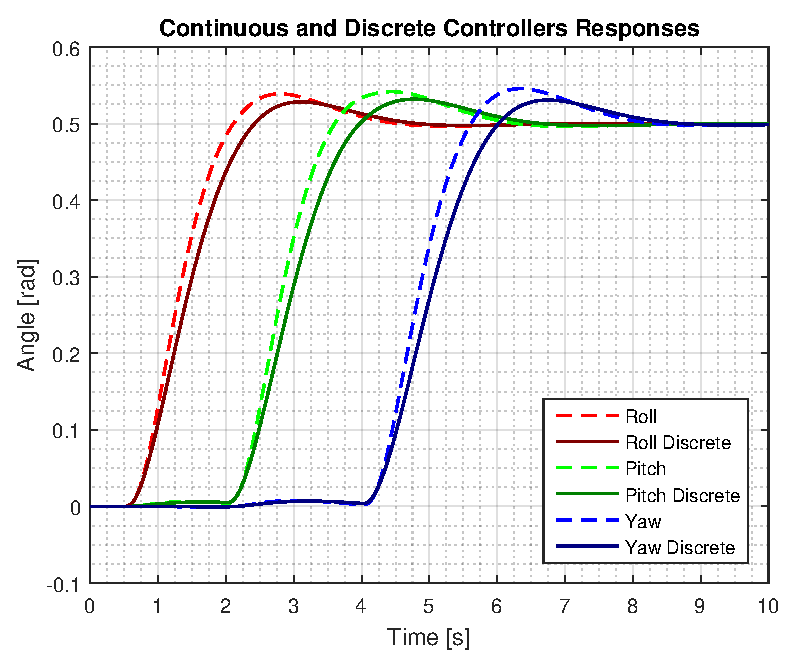
\includegraphics[scale=0.65]{figures/simAttitudeDiscrete}
%	\caption{Attitude controller performance when discretized with a sampling rate of 28 Hz and its continuous version.}
%	\label{fig:AttitudeDiscrete}
%\end{figure}
%
%The discrete attitude controller is also evaluated by its control action, which is depicted in \autoref{fig:AttitudeDiscreteControlAction}. As it can be appreciated, the variations from equilibrium of the motor rotational speeds are larger in the discrete controller and the signals are away from equilibrium for a longer time.
%\begin{figure}[H]
%	\centering
%	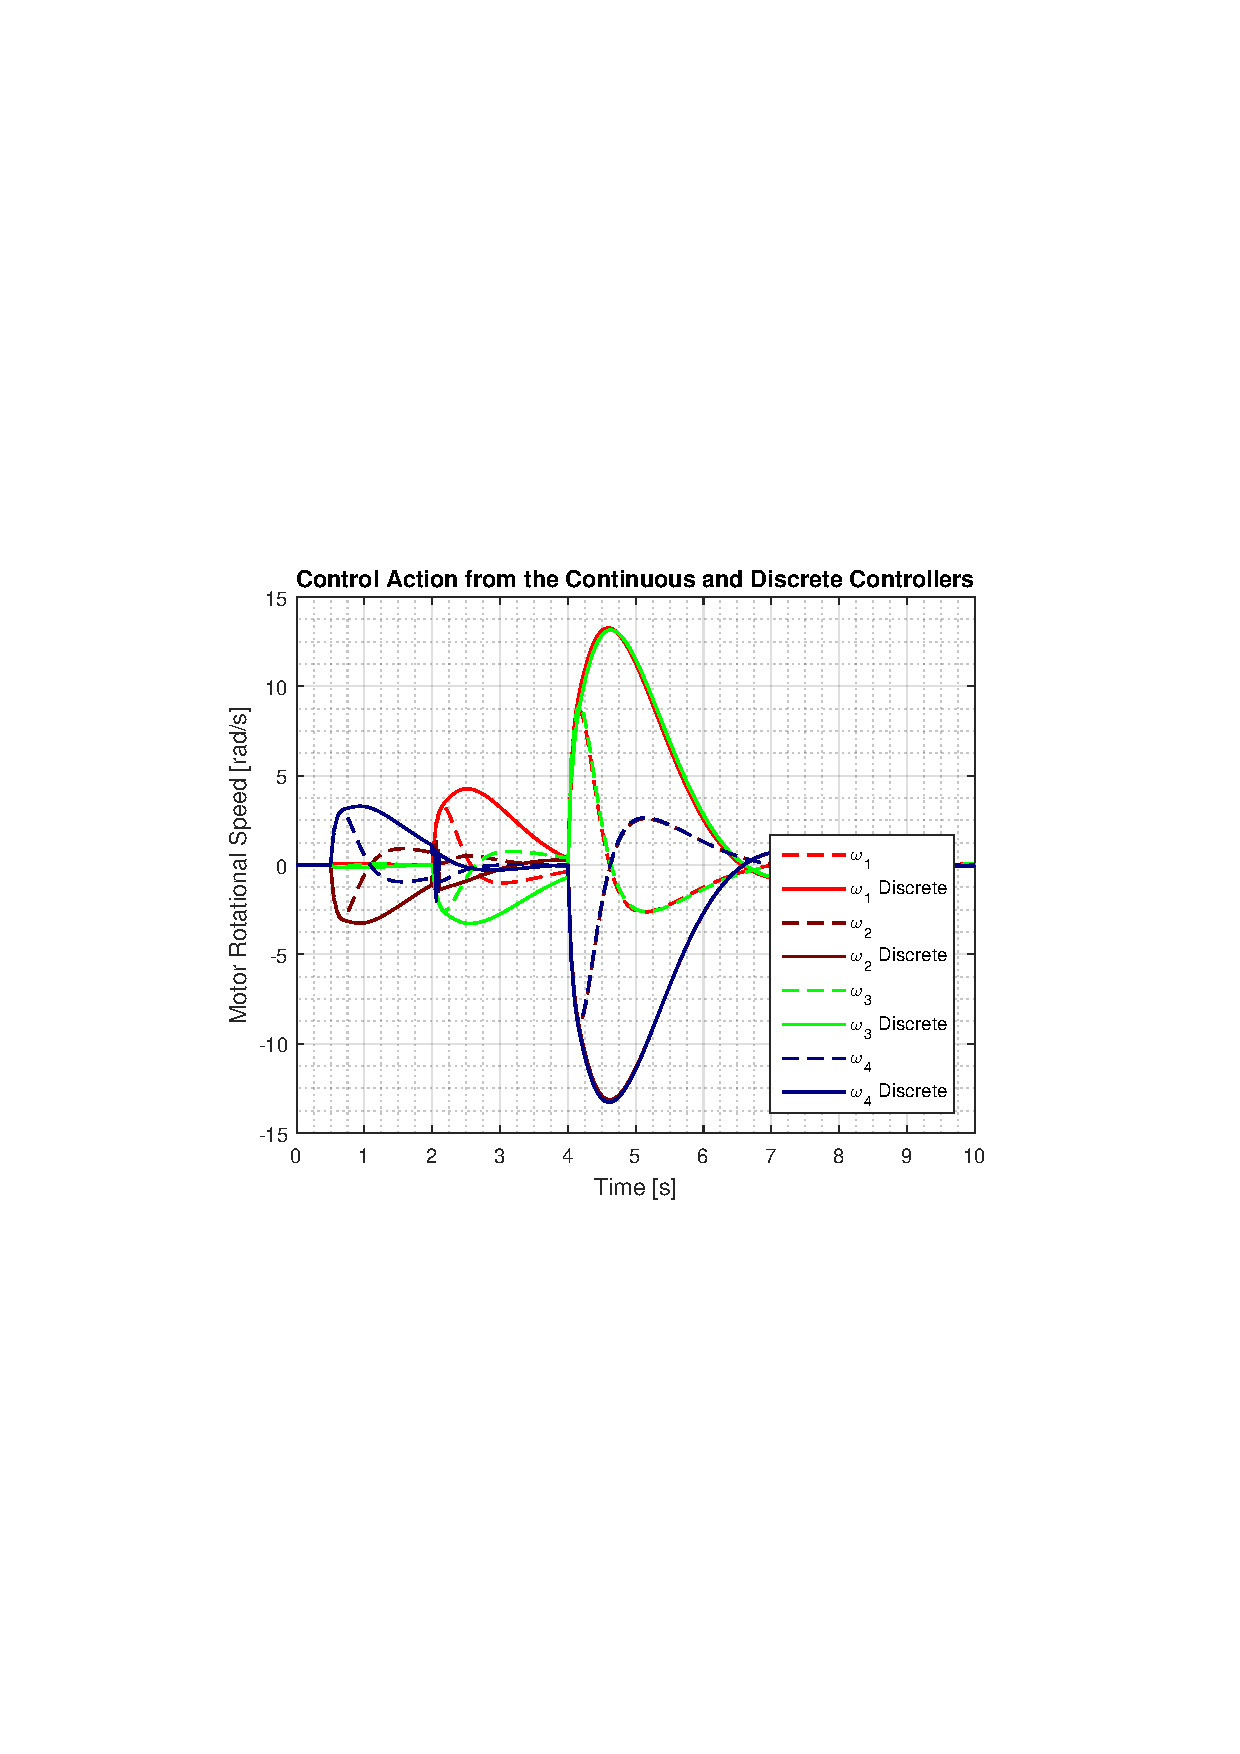
\includegraphics[scale=0.65]{figures/simAttitudeDiscreteControlAction}
%	\caption{Attitude controller control action when discretized with a sampling rate of 28 Hz and its continuous version.}
%	\label{fig:AttitudeDiscreteControlAction}
%\end{figure}
 
\subsection{Translational Controllers}
The translational position controllers contain only proportional terms, which means that no discretization is needed. However, the velocity controllers also include an integral terms so the need to be discretized. This is done using the same method as the attitude controller, the Tustin approximation.

The discrete versions of the PI controllers are 
\begin{flalign}
	\theta(k&)= \theta(k-1) -204.6 e_{\dot{x}}(k) + 199 e_{\dot{x}}(k-1)
	\label{discreteVelocityXcontrollerdiferences}\\
	\phi(k)&= \phi(k-1) -204.6 e_{\dot{y}}(k) + 199 e_{\dot{y}}(k-1)
	\label{discreteVelocityYcontrollerdiferences}\\
	\omega_{sum}(k)&= \omega_{sum}(k-1) -204.6 e_{\dot{z}}(k) + 199 e_{\dot{z}}(k-1)
	\label{discreteVelocityZcontrollerdiferences}
\end{flalign}

\subsection{Code Implementation}
As in the case of the communication, the controller are included in a task that runs every sampling period $T=0.035$ms.

\begin{lstlisting}[style=customcpp,
caption={Code for the controller task.}, 
label=lst:controllerTask]
void Controllers(void *pvParameters)
{
	portTickType xLastWakeTime;
	xLastWakeTime = xTaskGetTickCount();
	
	while (1)
	{
		Controller();
		ApplyVelocities();
		vTaskDelayUntil(&xLastWakeTime, 35);
	}
	vTaskDelete(NULL);
}
\end{lstlisting}
For doing that, the time at which the task starts is stored, then the control code is executed and the calculated control actions are sent to the motor controllers in the form of a PWM signal.

The implementation of the difference equations inside the function Controller() can be seen in \autoref{lst:controllers}, in which three examples ($\dot{z}_{\mathrm{I}}$ controller, integration in the state space controller and in the observer) are presented.

\begin{lstlisting}[style=customcpp,
caption={Code for the controllers.}, 
label=lst:controllers]
...
u_z = -208.8*vel_e_k[i] + 198.2*vel_e_k1[i] + u_z;
...
xint_k[i] = T / 2 * (e_k[i] + e_k1[i]) + xint_k1[i];
...
oint_k[i] = T / 2 * (o_k[i] + o_k1[i]) + oint_k1[i];
...

\end{lstlisting}

The function ApplyVelocities() is in charge of mixing the control action of the attitude controller with the one coming from the $z_{\mathrm{I}}$ controller. Then the duties that correspond to the desired rotational speeds of the motor is calculated using the information of \autoref{app:duty} and the PWM signal is sent to the motor controllers.